\usepackage{comment}

\subsubsection*{Le matin :}
Une réunion à été faite :
\begin{itemize}
    \item Faire un réseau simple.
    \item Lui faire apprende la fonction $1/3\, x + 2/3\, y$.
    \item Ajouter du bruit.
\end{itemize}

\subsubsection*{L'après midi :}
Le réseau essaye une fonction toute simple:
\begin{equation}
    \frac{1}{3} \times x + \frac{2}{3} \times y
\end{equation}
Les poids $1/3$ et $2/3$ ont été choisit pour casser la simétrie.
On y rajoute une perturbation random equiprobable entre $-err$ et $err$.
On essaye de visualiser l'erreur d'apprentissage en fonction de $err$. \\
Un petit script à donc été codé afin de visialiser la variation de l'erreur d'aprentissage:

\begin{figure}[H]
    \center
    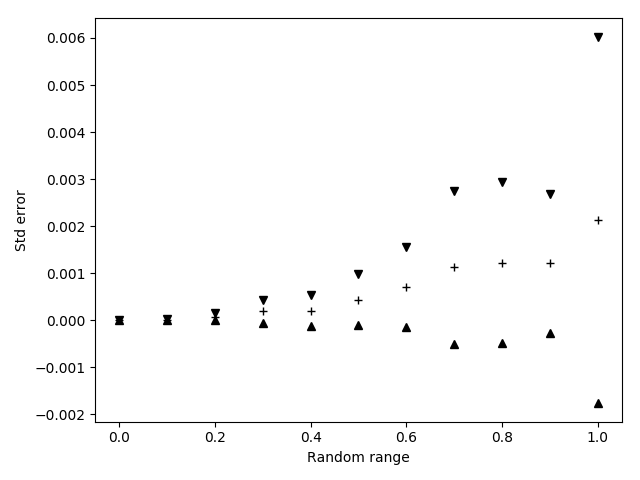
\includegraphics[height=\moyen]{sources/data/Obj2/tiers/graph1.png}
	\caption{Variation d'aprensitssage en fonction de la perturbation}
	\label{obj2tiers1}
\end{figure}

On peut voir que même si l'erreur moyenne augmente exponentiellement avec la perturbation,
elle reste très faible tant que la perturbation ne dépasse pas la moitié de la valeur théorique:
\begin{equation}
    err < 1/2 \; \; \; \Rightarrow \; \; \; R^2 > 0.999
\end{equation}
